\documentclass[a4paper,11pt]{article}

\usepackage[top=20mm,bottom=14mm,left=13mm,right=13mm,
  headheight=11mm,headsep=5mm]{geometry}
\usepackage{fontspec}
\usepackage{xeCJK}
\setmainfont{Times New Roman}
\setCJKmainfont{Yu Mincho}
\usepackage{microtype}
\usepackage{multicol}
\usepackage{enumitem}
\usepackage{fancyhdr}
\usepackage[table]{xcolor}
\usepackage{graphicx}
\usepackage{tabularx}
\usepackage{array}
\usepackage[hidelinks]{hyperref}

\definecolor{DeepBlue}{HTML}{1D4ED8}
\definecolor{RuleBlue}{HTML}{93C5FD}
\definecolor{SoftBlue}{HTML}{EFF6FF}
\definecolor{SoftCyan}{HTML}{ECFEFF}
\definecolor{SoftGray}{HTML}{F8FAFC}
\definecolor{Slate}{HTML}{475569}

\setlength{\parindent}{0.8em}
\setlength{\parskip}{0pt}
\setlength{\columnsep}{5mm}
\setlist[itemize]{leftmargin=1.2em,itemsep=0pt,topsep=1pt,parsep=0pt}
\setlist[enumerate]{leftmargin=1.4em,itemsep=0pt,topsep=1pt,parsep=0pt}
\renewcommand{\baselinestretch}{0.93}
\pagestyle{fancy}
\fancyhf{}
\fancyhead[C]{\officialheader}
\fancyfoot[C]{\small\thepage}
\renewcommand{\headrulewidth}{0pt}

\newcommand{\officialheader}{%
  \begin{minipage}[t]{\textwidth}
    \raggedleft{\small 氏名: ZHOU GUANJI}\par\vspace{0.5mm}
    \raggedleft
    {\small 試験区分: 情報科学区分,
    希望研究室: Internet Architecture and Systems Laboratory,
    現在の専門: Computer Science}\par
    \vspace{1.2mm}\hrule height 0.4pt
  \end{minipage}%
}

\newcommand{\majorsection}[1]{%
  \vspace{2pt}\noindent{\large\bfseries\color{DeepBlue} #1}\par\vspace{1pt}}
\newcommand{\subsectionrunin}[1]{%
  \vspace{1pt}\noindent{\bfseries\color{DeepBlue} #1}\par\nobreak\vspace{0pt}}
\newcommand{\figurecaption}[1]{%
  \par\vspace{1pt}\centering{\footnotesize\color{black} #1}\par\vspace{2pt}}
\newcommand{\tablecaption}[1]{%
  \par\vspace{3pt}\centering{\footnotesize\color{black} #1}\par\vspace{0pt}}

\begin{document}
\small

\noindent{\bfseries\color{DeepBlue} 取り組みたい研究テーマ：}
\color{black}
Evaluating Host-Level Context for Detecting Short-Lived DNS-over-HTTPS Traffic

\begin{multicols}{2}

\majorsection{1. これまでの修学内容}

My undergraduate thesis at the University of Science and Technology of China
studied robust TLS encrypted traffic classification under network
perturbation. The starting point was a weakness of
packet-length-sequence-based classifiers: although TLS hides payload contents,
packet lengths remain observable, yet they are affected by transport behavior.
Under congested network conditions, TCP-related dynamics
such as retransmission, sequence shift, and packet merging can change the
observed sequence. A classifier that relies on fixed packet positions may
therefore learn transport artifacts rather than
stable application-level patterns.

To address this issue, I designed TCP-Aware Contrastive Sequence (TAC-Seq), a
contrastive representation learning framework for perturbed packet-length
sequences, as shown in Figure~1. TAC-Seq was inspired by Rosetta's TCP-aware
traffic augmentation~\cite{rosetta}, but I redesigned the learning framework:
instead of reproducing Rosetta's BYOL-based approach, I used a SimCLR-style
objective with NT-Xent loss~\cite{simclr}. The augmentation pool modeled
subsequence repetition, subsequence shift, and Nagle-like packet-size
variation. In this design, disturbed observations of the same original flow are
used as related views, encouraging the model to learn features that remain
meaningful under transmission-level variation.

\end{multicols}
\begin{center}
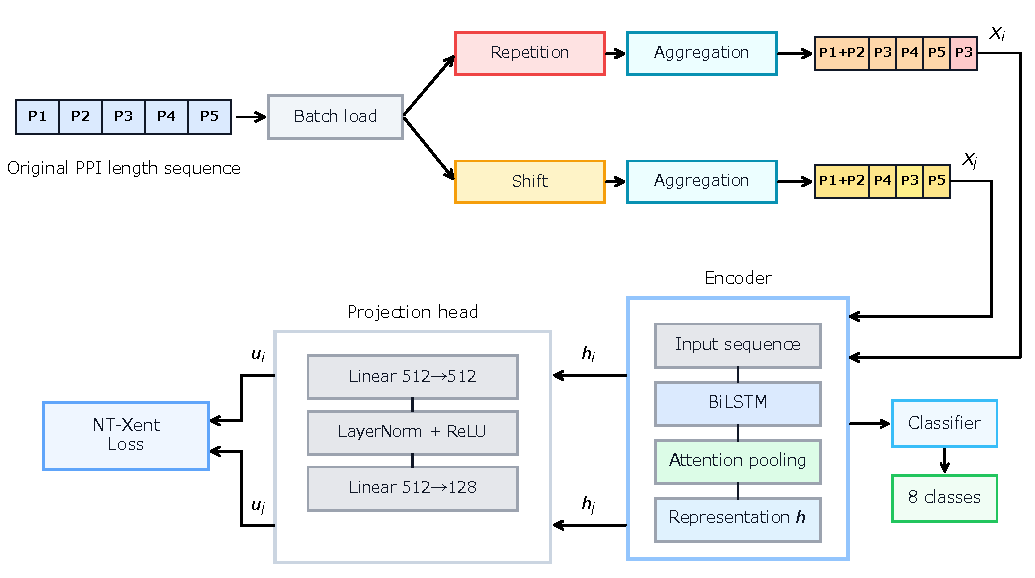
\includegraphics[width=0.75\textwidth]{assets/tacseq-framework-en.pdf}
\figurecaption{Figure 1. TAC-Seq framework implemented in my
undergraduate thesis.}
\end{center}
\begin{multicols}{2}

The model used self-supervised pretraining followed by downstream
classification. For sequence representation, TAC-Seq used a BiLSTM-Attention
encoder on packet-length sequences. During pretraining, two augmented views
from the same original flow formed a positive pair, while views from other
flows served as negative samples. The encoder output was passed through a
projection head for contrastive learning; after
pretraining, the projection head was removed and a classifier was trained on
top of the frozen encoder representation. This separation allowed me to
evaluate whether the encoder learned perturbation-robust sequence
representations, rather than only optimizing a classifier for one fixed setting.

The evaluation used CESNET-TLS22 with an eight-class TLS classification task.
To reflect an online classification setting, the input was
limited to packet-length information from the first 30 packets of each flow.
Robustness was tested under fixed FAST and RTO perturbation settings, and the
method was compared with a linear packet-length baseline and a Rosetta-style
implementation. I also disabled the packet-merging-related augmentation for
ablation. The results showed that TAC-Seq outperformed the linear baseline in
all settings and was stronger than the reproduced
Rosetta result in most settings, especially under more severe RTO
perturbations. Packet-size variation was useful in part of the evaluated
settings, particularly for lighter FAST perturbations. At the same time,
because the dataset did not provide timestamps, the Nagle-like component had
to be treated as a heuristic approximation rather than a protocol-exact
reconstruction. This limitation clarified that encrypted traffic analysis must
align model design with observable protocol evidence.

\majorsection{2. 取り組みたい内容}

\subsectionrunin{2.1 Background and problem.}
I would like to study practical security monitoring for encrypted traffic.
My initial project focuses on DNS over HTTPS (DoH). DoH protects DNS queries
by sending them over HTTPS~\cite{rfc8484}. This improves privacy, but it also
makes unauthorized DNS communication harder for a network operator to
identify because DoH can resemble ordinary web traffic.

Existing DoH detectors have made substantial progress. However, a recent
comparative analysis reports that some approaches depend on known resolver
addresses, traffic burstiness, or stable training conditions, while short or
single-query DoH flows to private resolvers remain difficult to
detect~\cite{jerabek2024}. This matters because malware can use a private
resolver and low-volume communication to reduce visibility.

The key difficulty is the unit of observation. A flow-level classifier sees
only a few encrypted packets in a short DoH flow, so it may not have enough
evidence unless it uses resolver identity or long-flow statistics. A monitored
host, however, may show temporal evidence around that flow, such as repeated
short HTTPS connections, short idle gaps, similar size--direction exchanges, or
changes in low-volume flow density within a short window, rather than relying
on one sparse flow sequence. This keeps the additional evidence tied to the
same monitored host. This motivates my research question:

\textit{Research question: Can host-level temporal context improve the
detection of short-lived DoH traffic to unseen private resolvers without
inspecting payloads or relying on resolver addresses?}

This question fits the Internet Architecture and Systems Laboratory's practical
direction. Katsura et al.\ showed that host-level aggregation can reduce IDS
cost while maintaining high accuracy in IoT networks~\cite{katsura2025}. I
will test this viewpoint when individual encrypted flows contain insufficient
information.

\subsectionrunin{2.2 Observation unit and feature design.}
The proposed method changes the analysis unit from an isolated TLS flow to a
host observation window. Each flow is represented by size, direction,
inter-arrival-time, duration, and count metadata; each candidate flow is paired
with a host window ending at the flow or at a specified detection delay.

The window statistics are derived from evidence missing in a short flow:
short-flow counts, temporal spacing, burst and idle patterns, repeated
size--direction profiles, and the share of low-volume encrypted communication.
These interpretable groups will be ablated independently, so the study tests
whether context supplies evidence rather than hiding resolver-specific
shortcuts inside a larger model.

\begin{center}
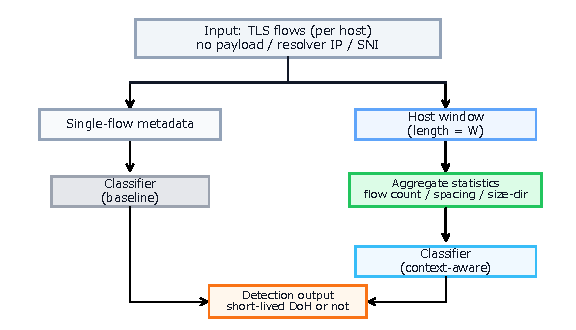
\includegraphics[width=0.98\columnwidth]{assets/doh-host-context-en.pdf}
\figurecaption{Figure 2. Flow-level and host-window observation units for
short-lived DoH traffic.}
\end{center}

\subsectionrunin{2.3 Testbed and baselines.}
I will construct a controlled testbed that captures ordinary HTTPS, benign DoH
to public resolvers, and low-volume DoH to private resolvers, including short
and single-query-like patterns. Collection will be repeated across separate
sessions and network conditions. Labeled traces will be split by resolver and
collection session, because a random flow-level split could place nearly
identical traffic in both sets and produce an optimistic result.

Model inputs will be limited to metadata outside encryption. Payloads, resolver
IP addresses, DNS names, SNI, ALPN, certificate subject names, and other
semantic TLS handshake fields will be excluded; TLS handshake packets may
contribute only size, direction, and timing. The host identifier is used only
to group flows into windows, not as a learned feature.

\subsectionrunin{2.4 Evaluation plan.}
The first comparison will use an address-list detector, a single-flow metadata
classifier, and a lightweight host-level model using the window statistics
above. The address-list result will be reported separately because it uses
resolver identity and cannot recognize unseen private resolvers. Representation
learning will be introduced only if simple aggregation fails to capture stable
behavior.

Host-level aggregation has a trade-off. A longer observation window can
provide more context, but it may also delay detection and combine unrelated
HTTPS connections. I will therefore evaluate multiple window sizes and query
frequencies. I will also add controlled delay and packet loss. The main
metrics will be recall for short-lived DoH flows, false-positive rate on
ordinary HTTPS traffic, F1 score, detection latency, memory use, and
processing time.

\begin{center}
\renewcommand{\arraystretch}{1.12}
\arrayrulecolor{RuleBlue}
\begin{tabularx}{0.98\columnwidth}{|>{\bfseries\scriptsize}p{8mm}|>{\scriptsize}X|}
  \hline
  RQ1 & Does host-level context improve recall compared with a single-flow
  model for short-lived DoH traffic? \tabularnewline \hline
  RQ2 & Does the improvement remain when the private resolvers used for
  testing are absent from the training data? \tabularnewline \hline
  RQ3 & How do the observation window, network conditions, latency, and
  false-positive rate affect deployment practicality? \tabularnewline \hline
\end{tabularx}
\arrayrulecolor{black}
\tablecaption{Table 1. Research questions and evaluation viewpoints.}
\end{center}

RQ1 compares flow-level and host-level models under the same metadata
restrictions. RQ2 uses disjoint resolver sets and collection sessions. RQ3
varies window size, query frequency, delay, and packet loss. Feature groups
will be removed in turn to identify which context supplies evidence.

\begin{center}
\renewcommand{\arraystretch}{1.11}
\arrayrulecolor{RuleBlue}
\begin{tabularx}{0.98\columnwidth}{|>{\bfseries\scriptsize\raggedright\arraybackslash}p{17mm}|>{\scriptsize\raggedright\arraybackslash}p{22mm}|>{\scriptsize\raggedright\arraybackslash}X|}
  \hline
  Variable & Controlled settings & Purpose \tabularnewline \hline
  Resolver & public / private; seen / unseen & Avoid learning a resolver-specific
  shortcut. \tabularnewline \hline
  Query form & single query / low rate / ordinary & Measure the difficult
  short-flow cases. \tabularnewline \hline
  Network & baseline / added delay / packet loss & Test robustness under changing
  conditions. \tabularnewline \hline
  Window & multiple durations & Quantify the recall--latency trade-off.
  \tabularnewline \hline
\end{tabularx}
\arrayrulecolor{black}
\tablecaption{Table 2. Controlled variables in the proposed evaluation.}
\end{center}

\subsectionrunin{2.5 Research stages and feasibility.}
The stages are: build a reproducible traffic-generation pipeline and reproduce
a simple flow-level baseline; measure its limits and evaluate interpretable
host-level statistics; and introduce representation learning only if simple
aggregation does not capture stable behavior. This order keeps the project
feasible and produces useful measurements even if the host-level model provides
only a limited improvement.

\subsectionrunin{2.6 Expected contribution and extension.}
The expected contribution is a reproducible comparison of flow-level and
host-level detection, including failure cases. The project does not assume that
all DoH traffic is detectable from metadata; it will clarify when host context
helps, which context features matter, and whether a lightweight detector is
practical. Newer transports such as DNS over QUIC (DoQ)~\cite{rfc9250} will be
reserved as later extensions.

\subsectionrunin{2.7 Scope and validation criteria.}
This proposal changes the unit of analysis from a single TLS flow to a host
observation window, so it does not simply repeat my undergraduate study. The
approach will be useful only if it improves short-lived DoH detection for
unseen resolvers while keeping false positives, latency, and processing cost
measurable. If improvement requires resolver identity, semantic handshake
fields, or an impractically long window, I will report that limitation and
preserve the settings, splits, and scripts needed to reproduce it.

\renewcommand{\refname}{\normalsize References}
\begin{thebibliography}{9}
\setlength{\itemsep}{0pt}
\setlength{\parsep}{0pt}
\footnotesize

\bibitem{rosetta}
R. Xie et al., ``Rosetta: Enabling Robust TLS Encrypted Traffic
Classification in Diverse Network Environments with TCP-Aware Traffic
Augmentation,'' USENIX Security, 2023.

\bibitem{simclr}
T. Chen et al., ``A Simple Framework for Contrastive Learning of Visual
Representations,'' ICML, 2020.

\bibitem{rfc8484}
P. Hoffman and P. McManus, ``DNS Queries over HTTPS (DoH),'' IETF RFC
8484, 2018.

\bibitem{jerabek2024}
M. Jerabek et al., ``Comparative Analysis of DNS over HTTPS Detectors,''
\emph{Computer Networks}, 2024.

\bibitem{katsura2025}
Y. Katsura et al., ``Efficient IDS for IoT Networks Using Host-Based Data
Aggregation and Multi-Entropy Analysis,'' \emph{IEEE Access}, 2025.

\bibitem{rfc9250}
C. Huitema et al., ``DNS over Dedicated QUIC Connections,'' IETF RFC 9250,
2022.

\end{thebibliography}

\end{multicols}
\end{document}
